\documentclass[11pt]{article}

% ====================================================
% ====================================================
% USEPACKAGES AND IMPORTS
% ====================================================
% ====================================================

\usepackage[T1]{fontenc}
\usepackage[utf8]{inputenc}
\usepackage[english]{babel}

\usepackage[
	left=2.5cm,
  	right=2cm,
  	top=2.5cm,
  	bottom=4cm,
]{geometry}

\usepackage{tikz}
\usepackage{eso-pic}
\usepackage{fancyhdr}
\usepackage{etoolbox}
\usepackage{enumitem}
\usepackage{amssymb}
\usepackage{xparse}
\usepackage{roboto}
\renewcommand{\familydefault}{\sfdefault}

% definitions
% ====================================================

\let\titleoriginal\title
\renewcommand{\title}[1]{
	\titleoriginal{#1}
	\newcommand{\thetitle}{#1}
}

\setlength{\parskip}{\baselineskip}%
\setlength{\parindent}{0pt}%

% header and footer
\pagestyle{fancy}
\fancyhf{}
\lhead{\thetitle}
\rhead{
\includegraphics[width=2cm]{../03_img/logo_dhbw.png}}
\cfoot{\thepage\\\vspace{0.6cm} \small Applied Machine Learning Fundamentals}
\setlength{\headsep}{1.5cm}

% commands
% ====================================================

% title page theme
\newcommand\BackgroundPic{%
	\put(0,0){%
		\parbox[b][\paperheight]{\paperwidth}{%
			\vfill
			\centering
			\tikz[overlay,remember picture] \node[opacity=0.2, at=(current page.center)] {
				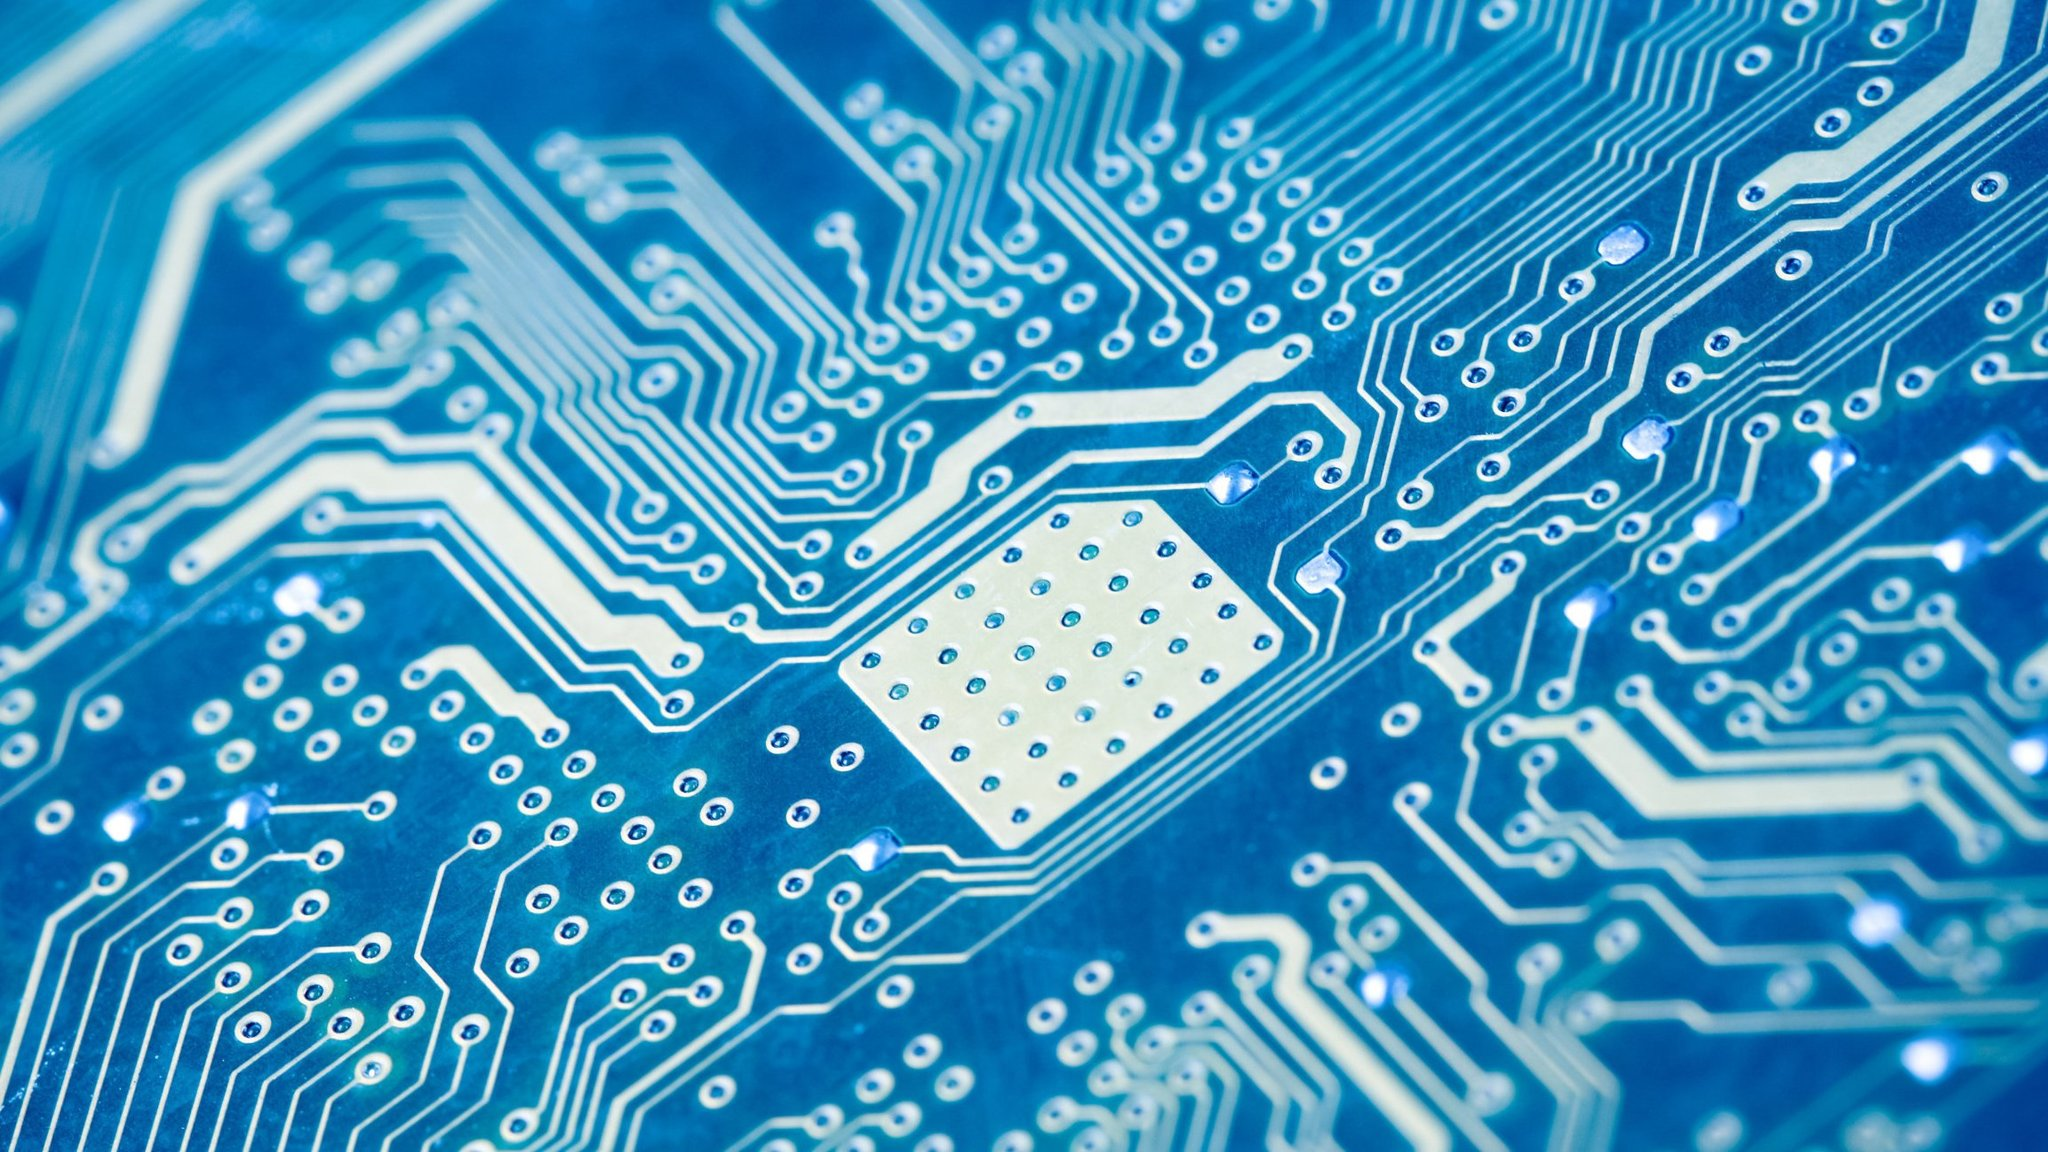
\includegraphics[height=\paperheight,width=\paperwidth]{../03_img/processor.jpg}
			};
			
\includegraphics[width=4cm, trim=-5.5cm 0 0 -1cm]{../03_img/logo_dhbw.png}
			\vfill
		}
	}
}

\newcommand\exercise[4][]{
	\ifx\hfuzz#1\hfuzz
  		\item #2\vspace{0.2cm}\newline #3 \vspace{#4}%
	\else
  		\item #2\vspace{0.2cm}\newline #3\vspace{0.5cm}\newline Solution:\newline#1 \vspace{#4}%
	\fi
}
